\begin{recipe}{Monkey Bread}{Serves 8}{3 hours and 45 minutes}
\freeform This recipe came from Sarah Younkin around Christmas, 2008.  Another huge crowd pleaser.  It is particular good to bring to a pot luck, preferable a brunch, but not necessarily.  People like it at night, too.
\newstep
Adjust oven rack to medium low position and heat to 200\0.  When oven reaches 200\0 turn it off.
\ing[2]{tbsp}{butter, unsalted, softened}
Butter a bundt pan and set aside.
\ing[2]{tbsp}{butter, unsalted, melted}
\ing[1]{c.}{milk, warm}
\ing[\fr13]{c.}{water, warm}
\ing[\fr14]{c.}{granulated sugar}
\ing[1]{pkg.}{rapid rise yeast}
In large measuring cup mix together.
\ing[3\fr14]{c.}{\apf{}}
\ing[2]{tsp}{salt}
Mix flour and salt in bowl of standing mixer fitted with dough hook.
\newstep
Turn machine to low and slowly add milk mixture.  After dough comes together, increase speed to medium and mix until dough is shiny and smooth, 6 to 7 minutes. Turn dough onto lightly floured surface and knead briefly to form smooth, round ball. Coat large bowl with oil. Place dough in bowl and coat surface of dough lightly with oil. Cover bowl with a kitchen towel and place in warm oven until dough doubles in size, 50 to 60 minutes.
\ing[1]{c.}{packed light brown sugar}
\ing[2]{tsp}{ground cinnamon}
\ing[8]{tbsp}{melted butter}
While the dough is rising, mix brown sugar and cinnamon together in bowl. Place melted butter in second bowl. Set aside.
\newstep
Gently remove dough from bowl and pat into rough 8-inch square. Using bench scraper or knife, cut dough into 64 pieces.
\newstep
Roll each piece of dough into a ball. Working a few at a time, dip balls in melted butter, then roll in brown sugar mixture. Layer balls in Bundt pan staggering seems where dough balls meet as you build layers.
\newstep
Cover bundt pan tightly with plastic wrap and place in turned off oven until dough balls are puffy and have risen 1 to 2 inches from the top of the pan, 50 to 70 minutes.
\newstep
Remove pan from oven and heat oven to 350 degrees. Unwrap pan and bake until top is deep borwn and caramel begins to bubble around edges, 30 to 35 minutes. Cool in pan for 5 minutes, then turn out onto platter and allow to cool slightly, about 10 minutes.
\ing[1]{c.}{powdered sugar}
\ing[2]{tbsp}{milk}
While the bread cools, whisk powdered sugar and milk in a small bowl until no lumps remain. Drizzle glaze over warm monkey bread and serve warm. 
\end{recipe}
\begin{figure}
\begin{center}
%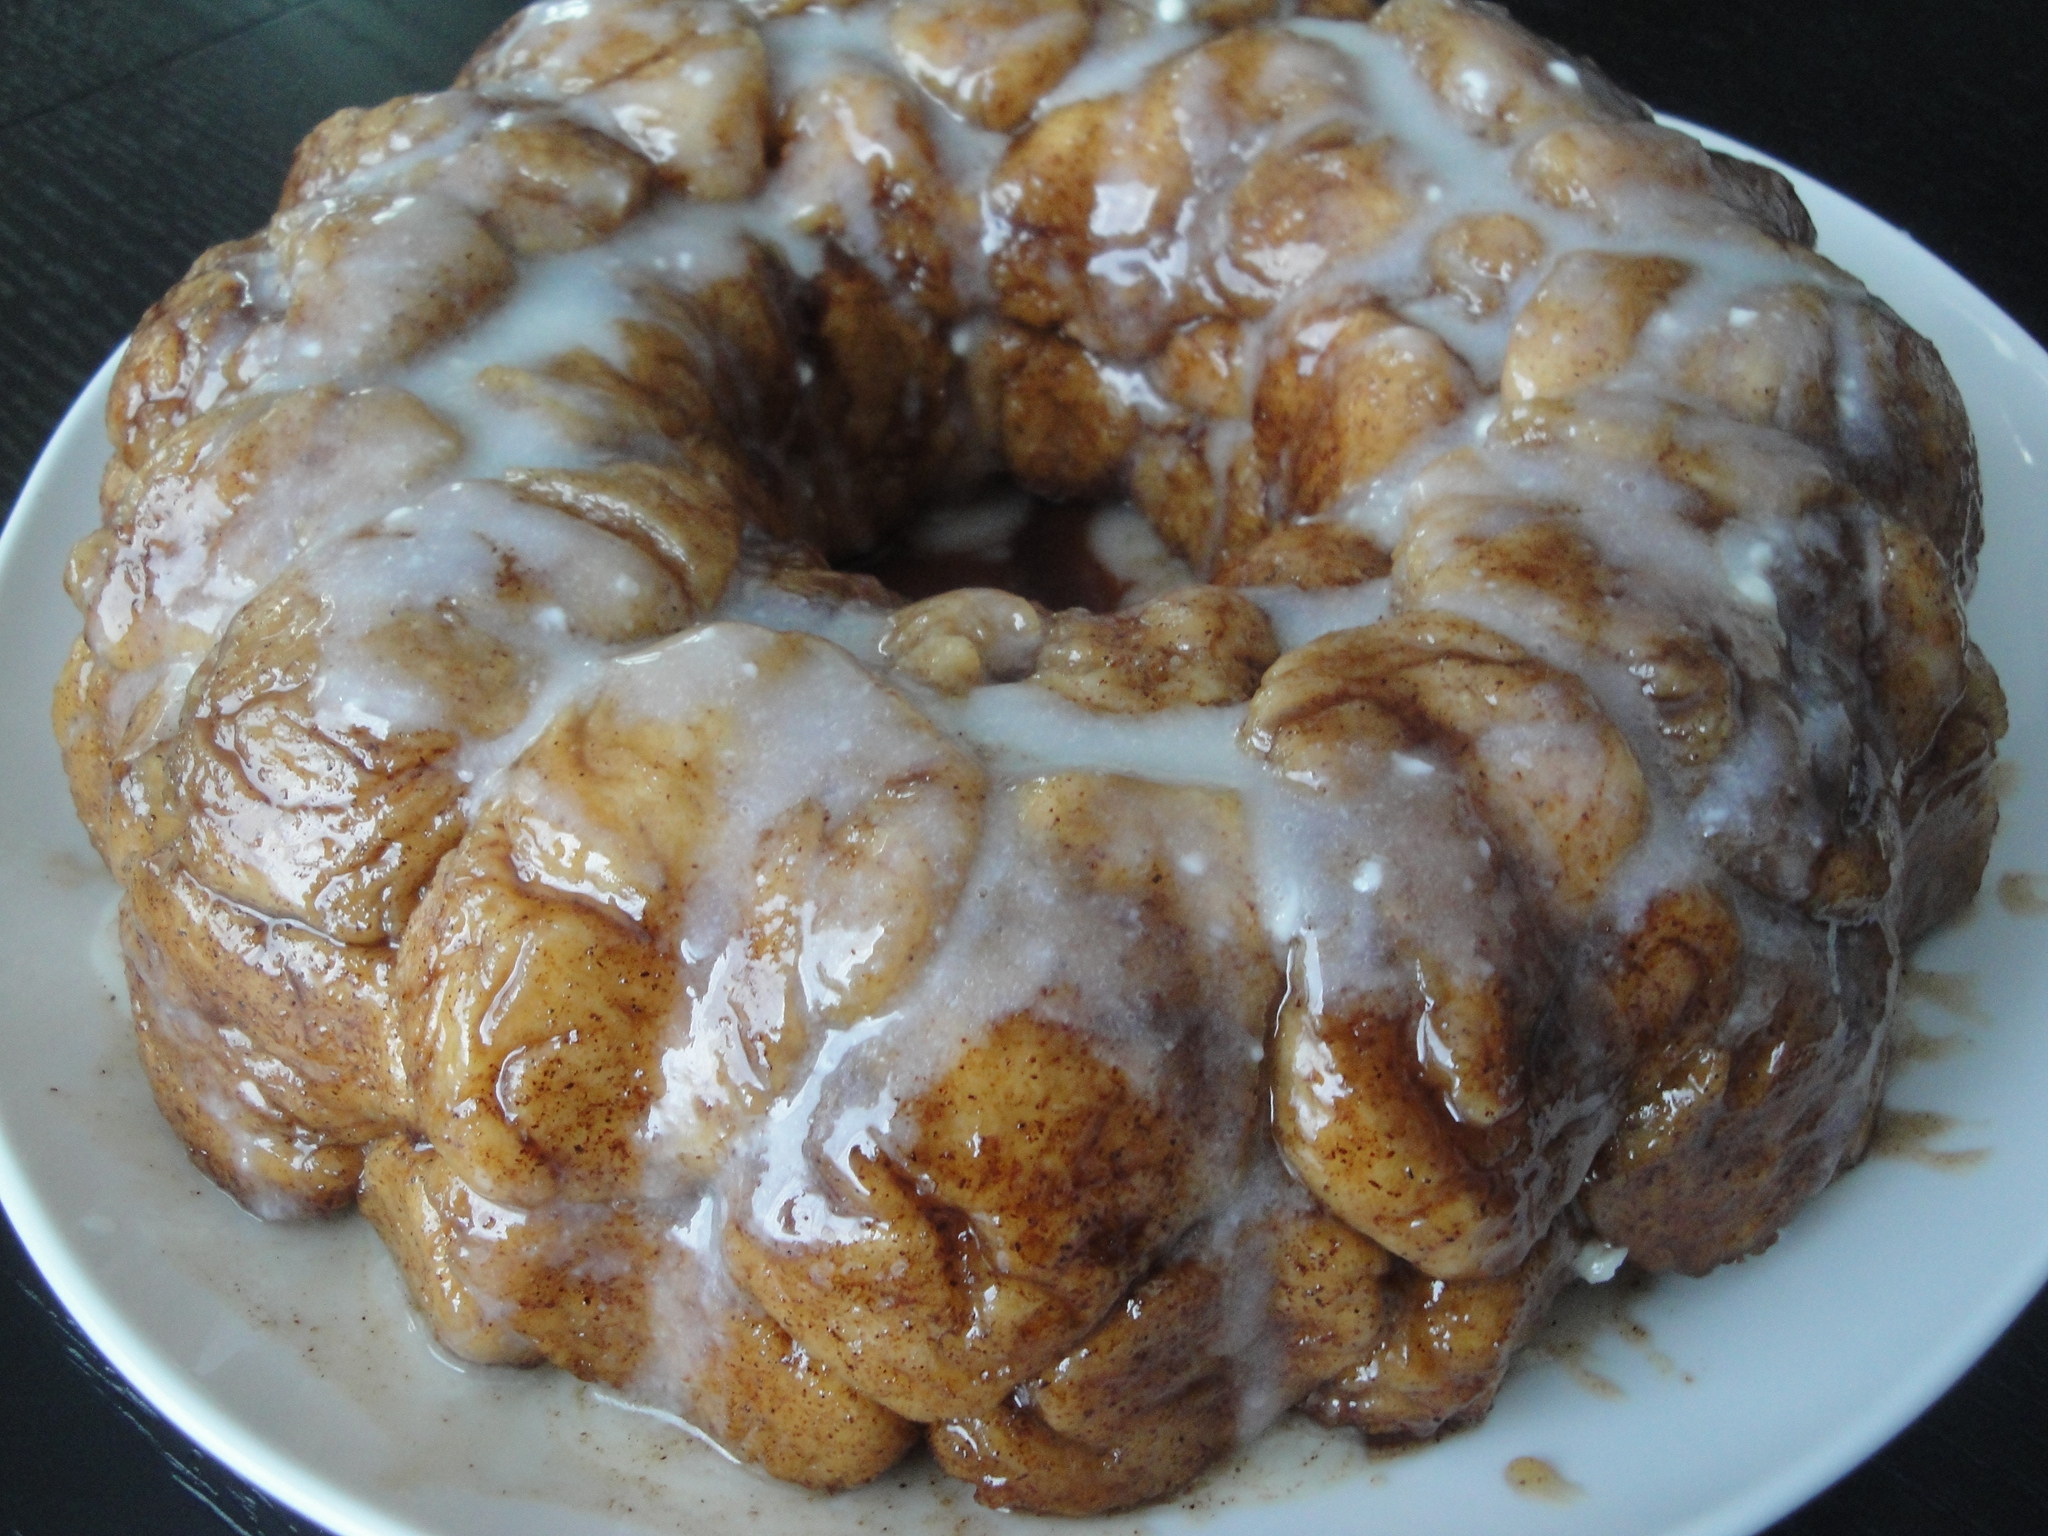
\includegraphics[width=0.8\textwidth]{monkey-bread}
%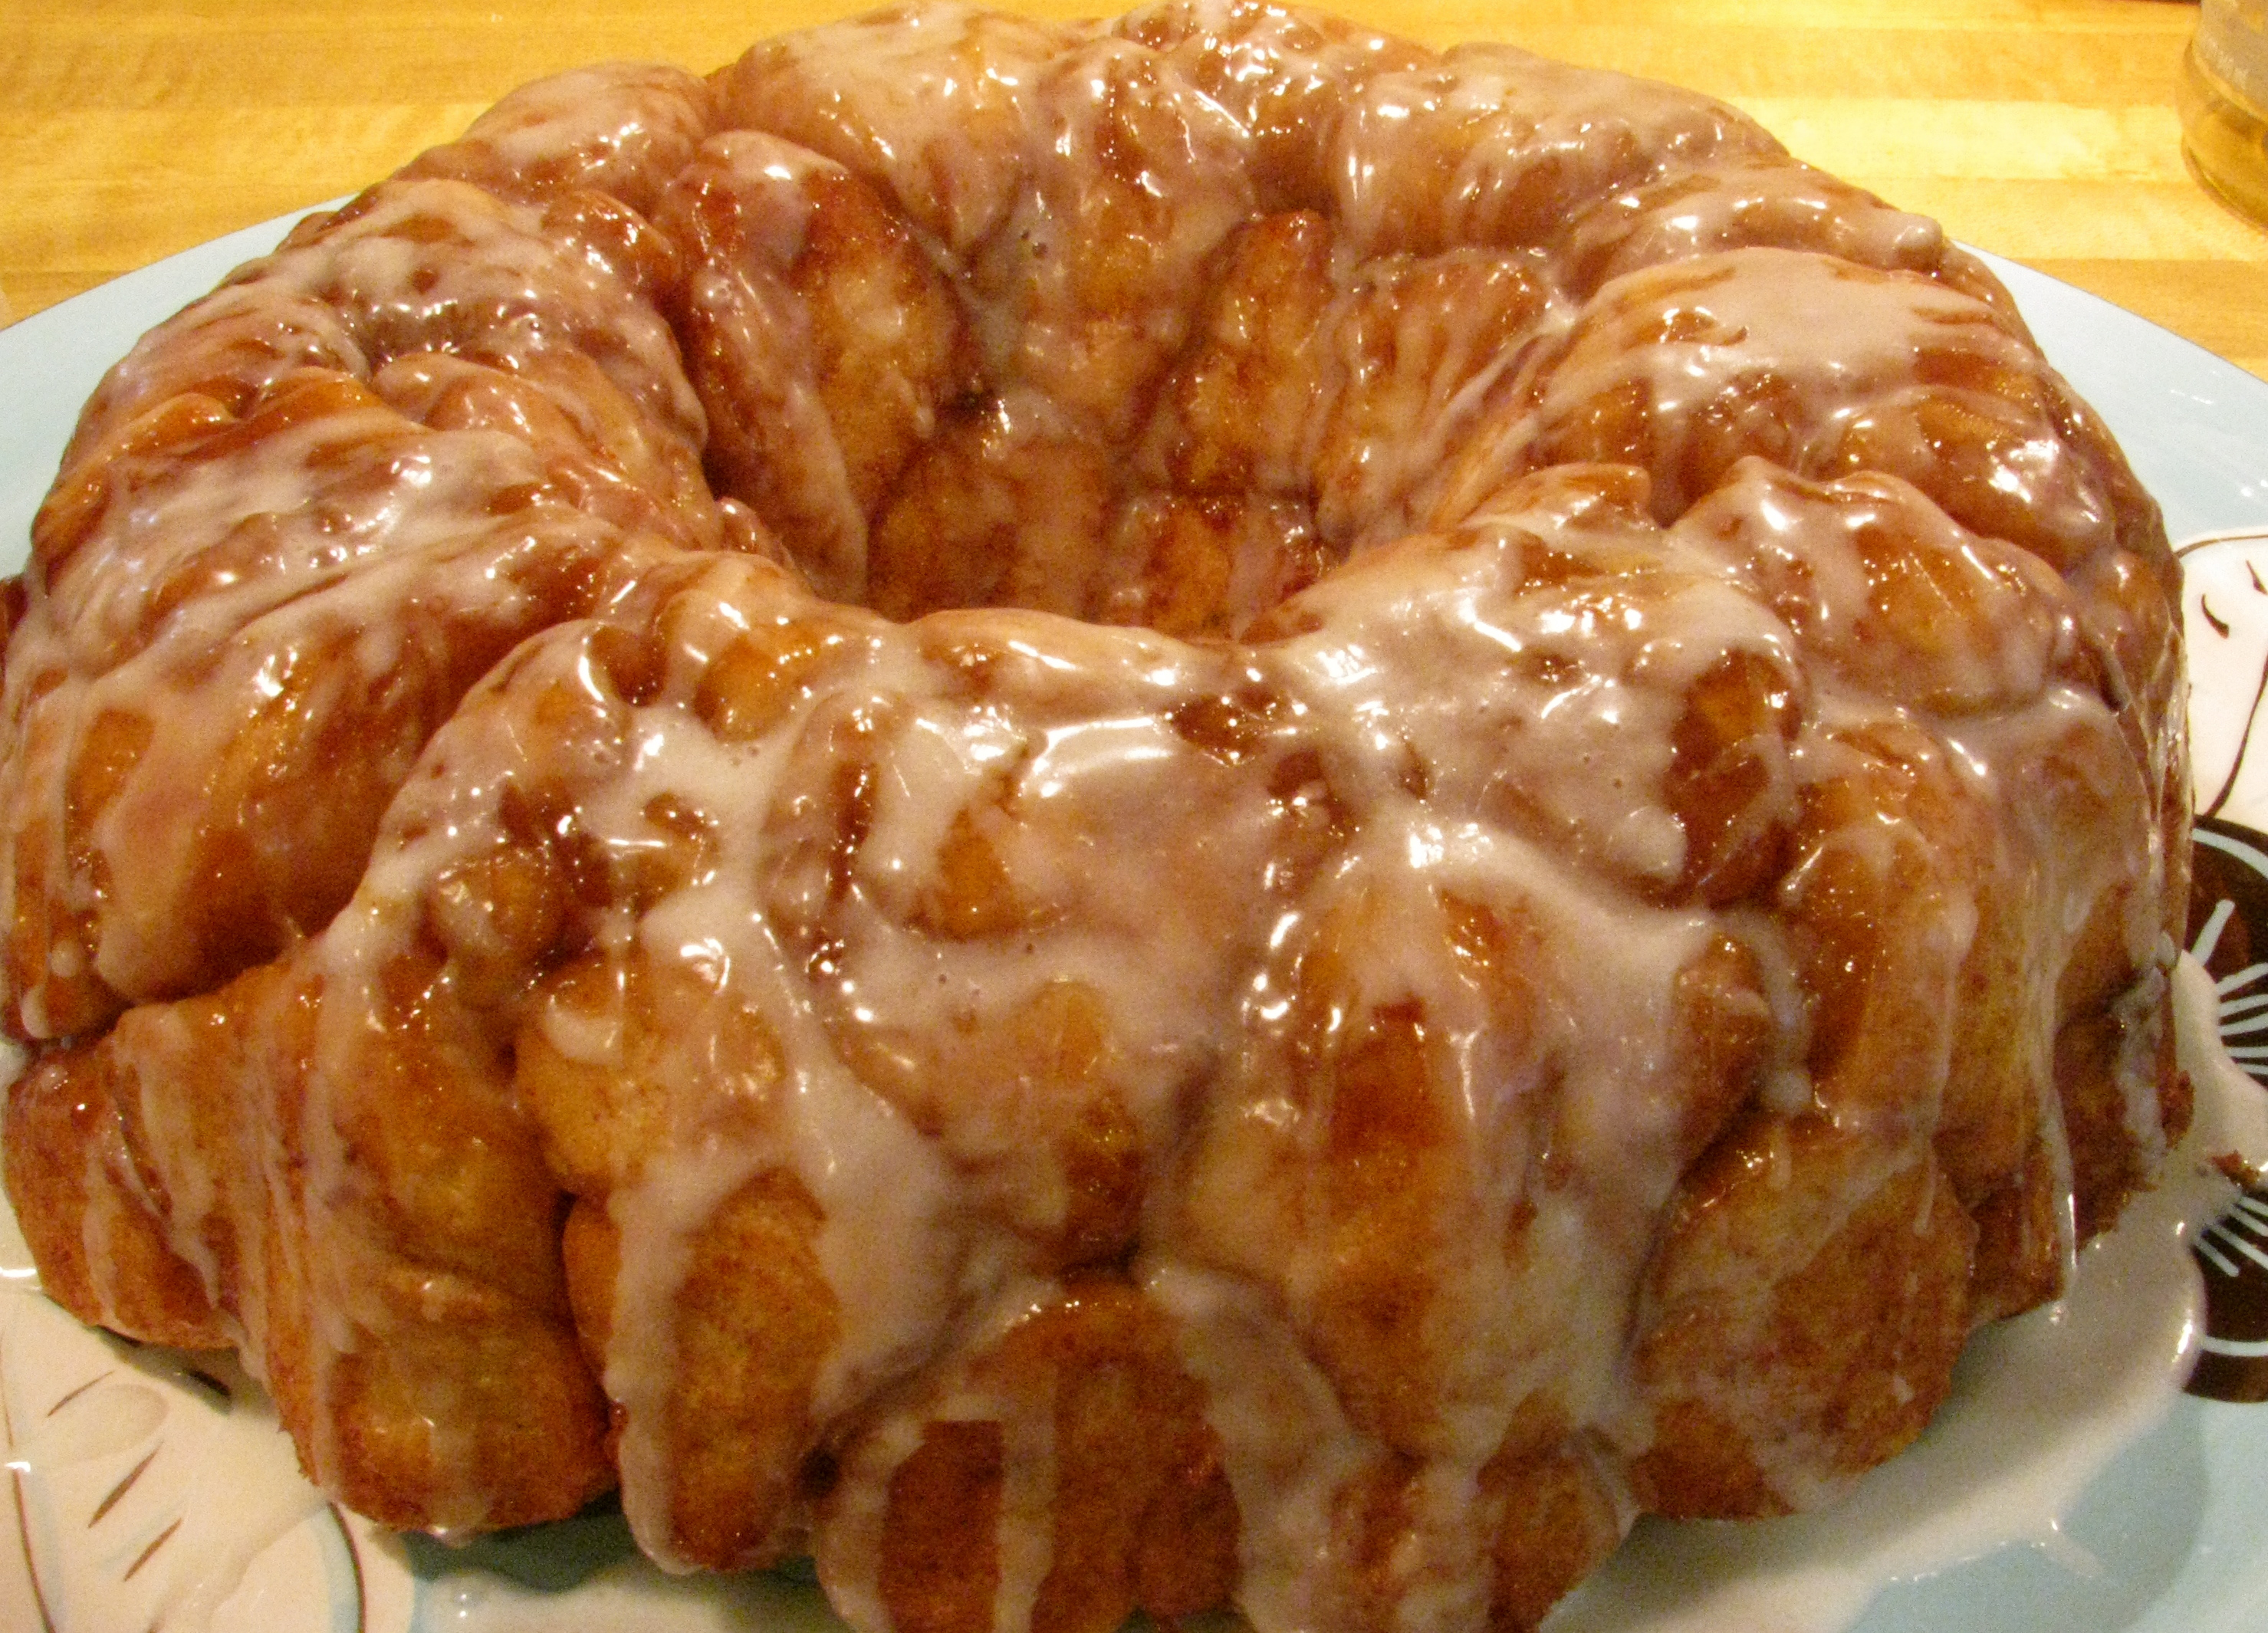
\includegraphics[width=0.3\textwidth]{/home/sgy/Dropbox/cookbook/figures/monkey-bread-2}
%\hspace{0.1\textwidth}
%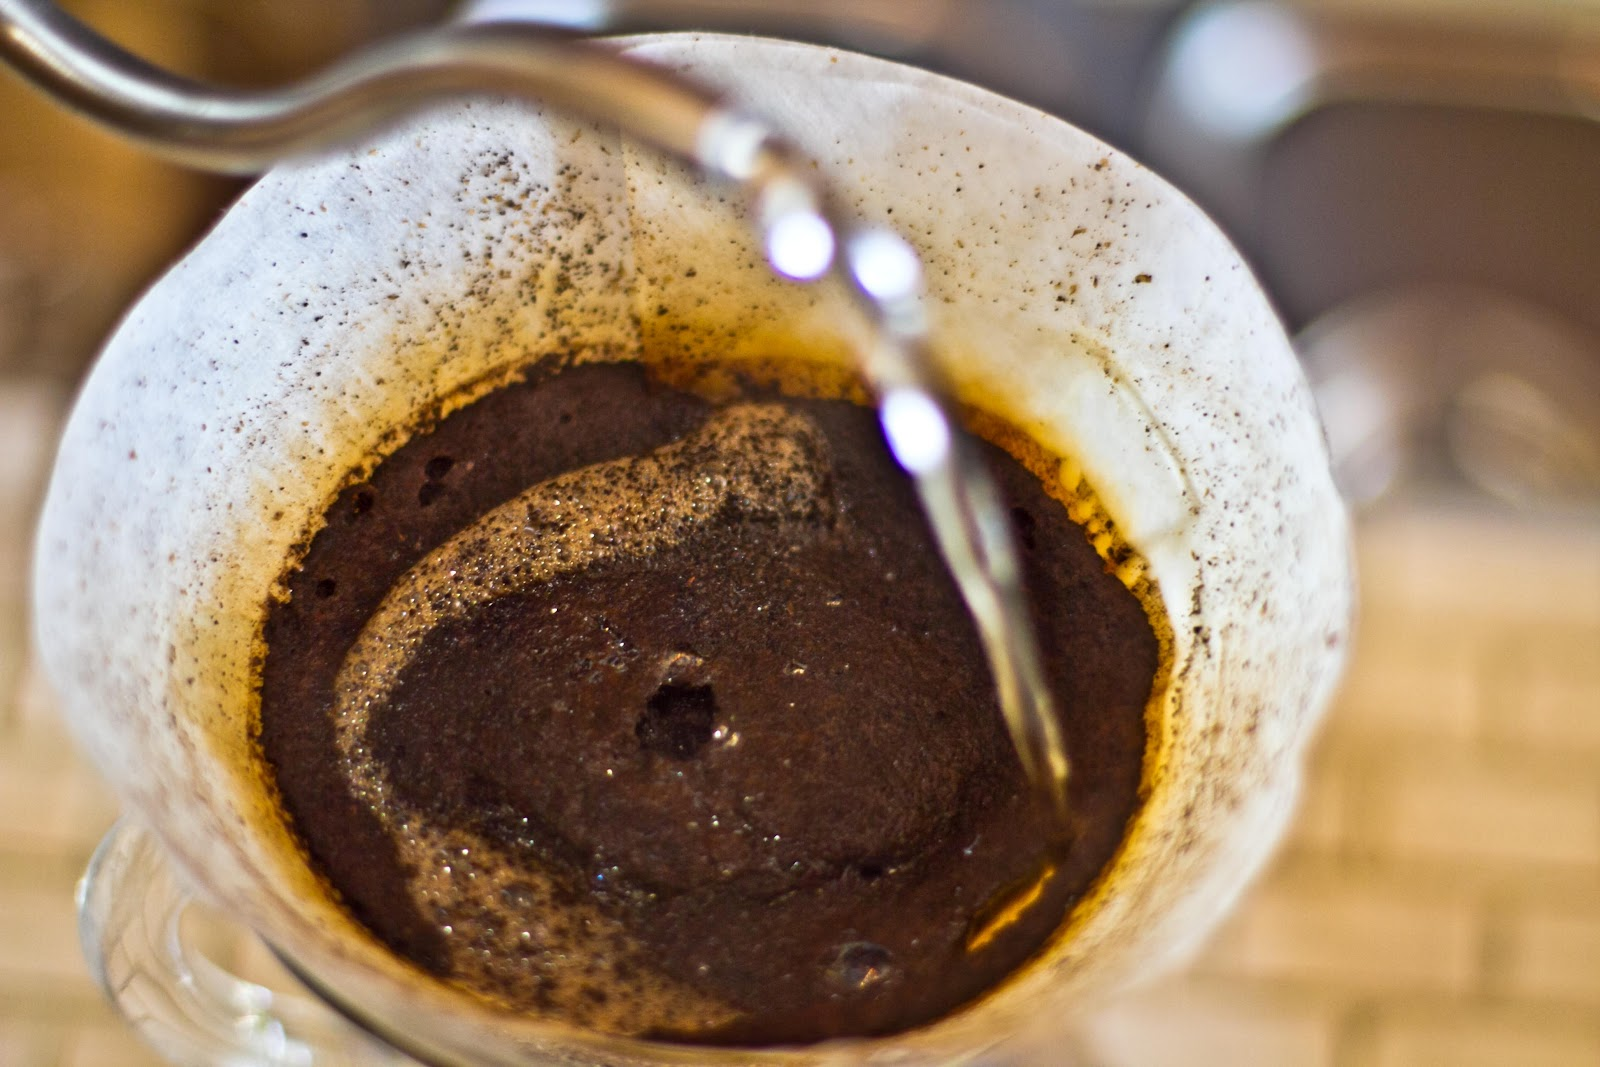
\includegraphics[height=0.25\textwidth]{chemex-2}
\end{center}
\caption*{Monkey bread}
\end{figure}
\clearpage
